\documentclass[12pt]{article}
\usepackage[top=1in,left=1in, right = 1in, footskip=1in]{geometry}

\usepackage{graphicx}
%\usepackage{adjustbox}

\usepackage{xcolor}
\usepackage{lineno}\renewcommand\thelinenumber{\color{gray}\arabic{linenumber}}
\linenumbers

\newcommand{\eref}[1]{Eq.~\ref{eq:#1}}
\newcommand{\fref}[1]{Fig.~\ref{fig:#1}}
\newcommand{\Fref}[1]{Fig.~\ref{fig:#1}}
\newcommand{\sref}[1]{Sec.~\ref{#1}}
\newcommand{\frange}[2]{Fig.~\ref{fig:#1}--\ref{fig:#2}}
\newcommand{\tref}[1]{Table~\ref{tab:#1}}
\newcommand{\tlab}[1]{\label{tab:#1}}
\newcommand{\seminar}{SE\mbox{$^m$}I\mbox{$^n$}R}

\usepackage{amsthm}
\usepackage{amsmath}
\usepackage{amssymb}
\usepackage{amsfonts}

%\usepackage{lineno}
%\linenumbers

\usepackage[pdfencoding=auto, psdextra]{hyperref}

\usepackage{natbib}
\bibliographystyle{chicago}
\date{\today}

\usepackage{xspace}
\newcommand*{\ie}{i.e.\@\xspace}

\usepackage{color}

\usepackage{xspace}
\newcommand{\Rx}[1]{\ensuremath{{\mathcal R}_{#1}}} 
\newcommand{\Ro}{\Rx{0}\xspace}
\newcommand{\RR}{\ensuremath{{\mathcal R}}}
\newcommand{\Rhat}{\ensuremath{{\hat\RR}}}
\newcommand{\tsub}[2]{#1_{{\textrm{\tiny #2}}}}

\newcommand{\comment}[3]{\textcolor{#1}{\textbf{[#2: }\textsl{#3}\textbf{]}}}

%% \newcommand{\rev}[1]{\comment{red}{REV}{#1}}
\newcommand{\rev}[1]{}

\newcommand{\swp}[1]{\comment{magenta}{SWP}{#1}}
\newcommand{\jd}[1]{\comment{magenta}{JD}{#1}}
\newcommand{\bmb}[1]{\comment{magenta}{BMB}{#1}}
\newcommand{\dc}[1]{\comment{magenta}{DC}{#1}}
\newcommand{\jsw}[1]{\comment{magenta}{JSW}{#1}}
\newcommand{\mli}[1]{\comment{magenta}{MLi}{#1}}
\newcommand{\new}[1]{\textcolor{blue}{#1}}

\begin{document}

\begin{flushleft}{
	\Large
	\textbf\newline{
		Reconciling early-outbreak preliminary estimates of the basic reproductive number and its uncertainty: a new framework and applications to the novel coronavirus (2019-nCoV) outbreak
	}
}
\newline
\\
Sang Woo Park\textsuperscript{1,*}
David Champredon\textsuperscript{2}
David J.\,D.\ Earn\textsuperscript{3,4}
Michael Li\textsuperscript{5}
Joshua S. Weitz\textsuperscript{6, 7}
Bryan T. Grenfell\textsuperscript{1,8,9}
Jonathan Dushoff\textsuperscript{3,4,5,*}
\\
\bigskip
\textbf{1} Department of Ecology and Evolutionary Biology, Princeton University, Princeton, NJ, USA
\\
\textbf{2} Department of Pathology and Laboratory Medicine, University of Western Ontario, London, Ontario, Canada
\\
\textbf{3} Department of Mathematics and Statistics, McMaster University, Hamilton, ON, Canada
\\
\textbf{4} M.\,G.\,DeGroote Institute for Infectious Disease Research, McMaster University, Hamilton, ON, Canada
\\
\textbf{5} Department of Biology, McMaster University, Hamilton, ON, Canada
\\
\textbf{6} School of Biological Sciences, Georgia Institute of Technology, Atlanta, GA, USA
\\
\textbf{7} School of Physics, Georgia Institute of Technology, Atlanta, GA, USA
\\
\textbf{8} Division of International Epidemiology and Population Studies, Fogarty International Center, National Institutes of Health, Bethesda, MD, USA
\\
\textbf{9} Woodrow Wilson School of Public and International Affairs, Princeton University, Princeton, NJ, USA
\\
\bigskip

*Corresponding authors: swp2@princeton.edu and dushoff@mcmaster.ca
\end{flushleft}

\section*{Abstract}
A novel coronavirus (2019-nCoV) has recently emerged as a global threat. 
As the epidemic progresses, many disease modelers have prioritized estimating the basic reproductive number \Ro, defined as the average number of secondary cases caused by a primary case.
While these efforts are extremely valuable, their modeling approaches and the resulting estimates vary widely.
Here, we present a framework for comparing different estimates of \Ro\ across a wide range of models by decomposing it into three key quantities (the exponential growth rate $r$, the mean generation interval $\bar G$, and the generation-interval dispersion $\kappa$) and apply our framework to early estimates of \Ro\ for the 2019-nCoV outbreak.
Our results emphasize the importance of propagating uncertainties in all three quantities, in particular in the shape of the generation-interval distribution.
While rapid response during an outbreak can be valuable, avoiding over-confidence is also important.
Modelers should work with field-workers to develop better methods for characterizing generation intervals.

\pagebreak

\section{Introduction}

Since December 2019, a novel coronavirus (2019-nCoV) has been spreading in China and other parts of the world \citep{pneumonia}.
Although the virus is believed to have originated from animal reservoirs \citep{cdcncov}, its ability to directly transmit between humans has posed a greater threat for its spread \citep{huang2020clinical,who26report}.
As of January 30th, 2020, the World Health Organization (WHO) has confirmed 7818 cases, including 82 confirmed cases in 18 different countries, outside China \citep{who28report}.
WHO has now declared the outbreak a Public Health Emergency of International Concern \citep{whoemer}.

As the disease continues to spread, many researchers have published analyses of the outbreak, focusing in particular on estimates of the basic reproductive number \Ro (i.e., the average number of secondary cases generated by a primary case in a fully susceptible population \citep{anderson1991infectious, diekmann1990definition}).
Estimating the basic reproductive number is of interest during an outbreak because it provides information about the level of intervention required to interrupt transmission \citep{anderson1991infectious}, and about the final size of the outbreak \citep{anderson1991infectious, ma2006generality}.
We commend these researchers for their timely contribution and those who made the data publicly available.
However, it can be difficult to assess the validity of the estimates of \Ro (as well as the associated degrees of uncertainty) when the estimation methods and their underlying assumptions vary widely, especially since these assumptions can affect the estimates.

Here, we show that a wide range of approaches to estimating \Ro\ can be understood and compared in terms of estimates for three quantities: the exponential growth rate $r$, the mean generation interval $\bar G$, and the generation-interval dispersion $\kappa$.
The generation interval, which is defined as the time between when an individual becomes infected and when that individual infects another individual \citep{svensson2007note}, plays a key role in shaping the relationship between $r$ and \Ro\ \citep{wearing2005appropriate, roberts2007model, wallinga2007generation, park2019practical};
therefore, estimates of $\mathcal R_0$ from different models directly depend on their implicit assumptions about the shape of the generation-interval distribution and the exponential growth rate.
Early in an epidemic, information is scarce and, inevitably, there is large uncertainty around case reports (affecting the estimates of the exponential growth rate) and contact tracing (affecting the estimates of the generation-interval distribution).
We suggest that disease modelers should make sure their assumptions about these three quantities are clear and reasonable, and that estimates of uncertainty should propagate error from all three sources.

We evaluate six disparate models published online between January 24--26, 2020 that estimated \Ro\ for the 2019-nCoV outbreak \citep{imaincov, liuncov, majumderncov, readncov, riouncov, zhaoncov}. 
We use our framework to construct pooled estimates for the three key quantities: $r$, $\bar G$, and $\kappa$. 
We use these pooled estimates to illustrate the importance of propagating different sources of error, particularly uncertainty in both the growth rate and the generation interval. 
We also use our framework to unravel which assumptions of these different models led to their different estimates and confidence intervals.

\section{Results}

\begin{table}[t]
\begin{center}
\scriptsize
\begin{tabular}{l|p{3.5cm}|p{2.5cm}|p{2.5cm}|l}
 & Basic reproductive\newline number \Ro\ & Mean generation\newline time $\bar G$ (days) & Generation interval\newline dispersion $\kappa$ \\
\hline
Study 1 & 2.5 (1.5--3.5)$^\ast$ & 8.4 & unspecified$^\dagger$ & \cite{imaincov} \\
\hline
Study 2 & 2.92 (95\% CI: 2.28--3.67) & 8.4 & 0.2 & \cite{liuncov} \\
\hline
Study 3 & 3.8 (95\% CI: 3.6--4.0) & 7.6 & 0.5 & \cite{readncov} \\
\hline
Study 4 & 2.2 (90\% CI: 1.4--3.8) & 7--14 & 0.5 & \cite{riouncov} \\
\hline
Study 5 & 5.47 (95\% CI: 4.16--7.10)$^\ddagger$ & 7.6--8.4 & 0.2 & \cite{zhaoncov} \\
\hline
Study 6 & 2.0--3.1 & 6--10 & 0 & \cite{majumderncov} \\
\hline
\end{tabular}
\end{center}
\caption{
\textbf{Reported estimates of the basic reproductive number and the assumptions about the generation-interval distributions.}
Estimates of \Ro and their assumptions about the shape of the generation interval distributions were collected from 6 studies.
$^\ast$We treat these intervals as a 95\% confidence interval in our analysis.
$^\dagger$We assume $\kappa = 0.5$ in our analysis.
$^\ddagger$The authors presented \Ro estimates under different assumptions; we use their baseline scenario in our analysis.
}
\end{table}

We gathered information on estimates of \Ro and their assumptions about the underlying generation-interval distributions from 6 articles that were published online between January 24th, 2020 and January 26th, 2020 (Table 1).
As most studies do not report their estimates of the exponential growth rate or the associated confidence intervals, we first recalculate the exponential growth rate that correspond their model assumptions.
We do so by modeling explicitly or implicitly reported distributions of the reproductive number \Ro, the mean generation interval $\bar G$, and the generation-interval dispersion parameter $\kappa$ with appropriate probability distributions;
we used Gamma distributions to model values reported with confidence intervals and uniform distributions to model values reported with ranges.
For example, Study 2 estimated $\Ro = 2.92$ (95\% CI: 2.28--3.67);
we model this estimate as a Gamma distribution with a mean of 2.92 and a shape parameter of 67, which has a 95\% probability of containing a value between 2.28 and 3.67 (see Table 2 for a complete description).
We then constructed a family of parameter sets -- which include $r$, $\bar G$, and $\kappa$ -- for each study and used these in a Bayesian multilevel model to build a distribution of pooled estimates (see Methods).

\newcommand{\gammdist}{\mathrm{Gamma}}
\begin{table}[t]
\begin{center}
\scriptsize
\begin{tabular}{l|p{4.5cm}|p{2.5cm}|p{2.5cm}}
 & Basic reproductive\newline number \Ro\ & Mean generation\newline time $\bar G$ (days) & Generation interval\newline dispersion $\kappa$  \\
\hline
Study 1 & $\gammdist(\mathrm{mean}=2.6, \alpha=28)$ & 8.4 & 0.5 \\
\hline
Study 2 & $\gammdist(\mathrm{mean}=2.92, \alpha=67)$ & 8.4 & 0.2 \\
\hline
Study 3 & $\gammdist(\mathrm{mean}=3.8, \alpha=1400)$ & 7.6 & 0.5 \\
\hline
Study 4 & $\gammdist(\mathrm{mean}=2.2, \alpha=12)$ & $\mathrm{Uniform}(7, 14)$ & 0.5\\
\hline
Study 5 & $\gammdist(\mathrm{mean}=5.47, \alpha=54)$ & $\mathrm{Uniform}(7.6, 8.4)$ & 0.2\\
\hline
Study 6 & $\exp(r \bar G)^\ast$ & $\mathrm{Uniform}(6, 10)$ & 0\\
\hline
\end{tabular}
\end{center}
\caption{
\textbf{Probability distributions for \Ro, $\bar G$, and $\kappa$.}
We use these probability distributions to obtain a probability distribution for the exponential growth rate $r$.
The Gamma distribution is parameterized by its mean and shape $\alpha$.
Constant values are fixed according to Table 1.
$^\ast$Study 6 uses the IDEA model \citep{fisman2013idea}, through which the authors effectively fit an exponential curve to the cumulative number of confirmed cases without propagating any statistical uncertainty.
Instead of modeling \Ro with a probability distribution and recalculating $r$, we use $r=0.114\,\mathrm{days}^{-1}$, which explains all uncertainty in \Ro they report, when combined with the range of $\bar G$ they consider.
}
\end{table}

\fref{assumption} compares the reported values of the exponential growth rate $r$, mean generation interval $\bar G$, and the squared coefficient of variation (CV) $\kappa$ of the generation-interval distribution from different studies with our pooled estimates ($\mu_r$, $\mu_G$, and $\mu_\kappa$) that we calculate from our multilevel model.
We find that there is a large uncertainty associated with the underlying parameters;
many models rely on stronger assumptions that ignore these uncertainties.
Surprisingly, no studies take into account how the variation in generation intervals affects their estimates of \Ro:
all studies assumed fixed values for $\kappa$, ranging from 0 to 0.5.
Assuming fixed parameter values can lead to overly strong conclusions \citep{elderd2006uncertainty}.
It is also interesting that none of the six studies explicitly or implicitly assumed an exponentially distributed generation interval (i.e., $\kappa=1$), an assumption which used to be extremely common, particularly implicitly.

\begin{figure}[t]
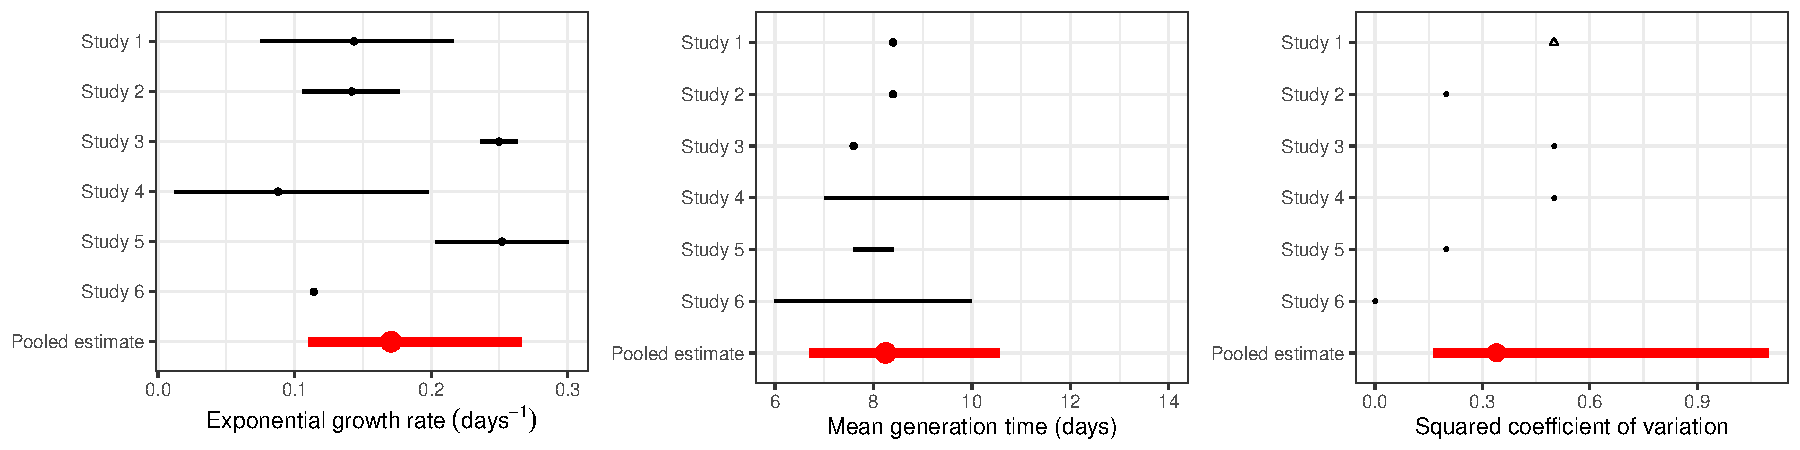
\includegraphics[width=\textwidth]{compare_assumption.pdf}
\caption{
\textbf{Comparisons of the reported parameter values with our pooled estimates.}
We inferred point estimates (black), uniform distributions (orange) or confidence intervals (purple) for each parameter from each study, and combined them into pooled estimates (red; see text).
Open triangle: we assumed $\kappa=0.5$ for Study 1 as they do not report their generation interval dispersion.
}
\label{fig:assumption}
\end{figure}

\fref{eff} shows how propagating uncertainty ($\mu_r$, $\mu_G$, and $\mu_\kappa$) in different combinations would affect estimates and CIs for \Ro. For illustrative purposes, we use our pooled estimates, which represent a reasonable proxy for the state of knowledge as of 26 January. 
Comparing the models that include only some sources of uncertainty to the ``all'' model, we see that propagating error from the growth rate (which all but one of the studies reviewed did) is absolutely crucial: the middle bar (\textbf{GI mean}), which lacks growth-rate uncertainty, is far too narrow.
Propagating error from the generation interval also has important effects.
Once these two are included, the impact of leaving out uncertainty in the dispersion is small, though noticeable, in this particular example.

\begin{figure}[!ht]
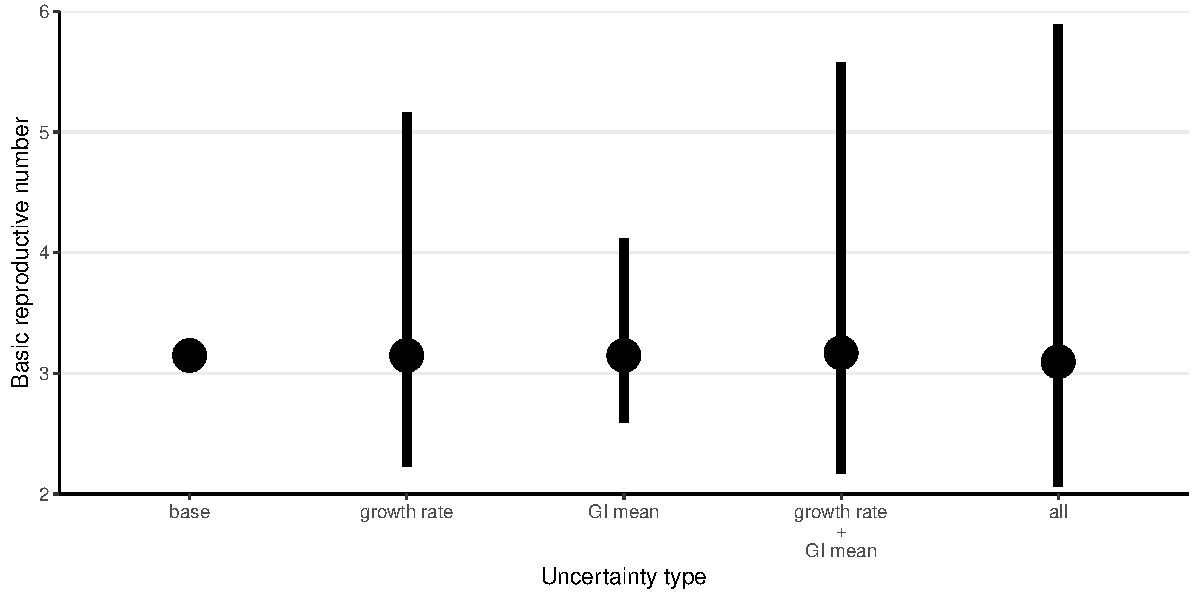
\includegraphics[width=\textwidth]{figure2.pdf}
\caption{
\textbf{Effects of $r$, $\bar G$, and $\kappa$ on the estimates of \Ro.}
We compare estimates of \Ro under five scenarios that propagate different combinations of uncertainties.
\textbf{base}: \Ro estimates based on the median estimates of $\mu_r$, $\mu_G$, and $\mu_\kappa$.
\textbf{growth rate}: \Ro estimates based on the the posterior distribution of $\mu_r$ while using median estimates of $\mu_G$ and $\mu_\kappa$.
\textbf{GI mean}: \Ro estimates based on the the posterior distribution of $\mu_G$ while using median estimates of $\mu_r$ and $\mu_\kappa$.
\textbf{growth rate + GI mean}: \Ro estimates based on the the joint posterior distributions of $\mu_r$ and $\mu_G$ while using a median estimate of $\mu_\kappa$.
\textbf{all}: \Ro estimates based on the joint posterior distributions of  $\mu_r$, $\mu_G$, and $\mu_\kappa$.
Vertical lines represent the 95\% confidence intervals.
}
\label{fig:eff}
\end{figure}

We also evaluate the estimates of \Ro across different studies by 
replacing their values of $r$, $\bar G$, and $\kappa$ with our pooled estimates ($\mu_r$, $\mu_G$, and $\mu_\kappa$) one at a time and recalculating the basic reproductive number \Ro (\fref{R0}).
We find that incorporating uncertainties one at a time increases the width of the confidence intervals all but three cases.
We estimate slightly narrower confidence intervals for Study 2 and Study 6 when we use our pooled estimate of the squared CV in generation time $\mu_\kappa$ to recalculate \Ro because they assume a narrow generation-interval distribution (compare \textbf{base} with \textbf{GI variation} in \fref{R0});
when higher values of $\kappa$ are used, their estimates of \Ro become less sensitive to the values of $r$ and $\bar G$, giving narrower confidence intervals.
We estimate narrower confidence intervals for Study 4 when we use our pooled estimate of the mean generation time $\mu_G$ to recalculate \Ro (compare \textbf{base} with \textbf{GI mean} in \fref{R0}) because the range of uncertainty in the mean generation time $\bar G$ they consider is much wider than the pooled range (\fref{assumption}).

Consistent with our previous observations (\fref{eff}),
we find that accounting for uncertainties in the estimate of $r$ has the largest effect on the estimates of \Ro (\fref{R0}).
For example, recalculating \Ro for Study 6 by using our pooled estimate of $r$ gives $\mathcal R_0 = 3.9$ (95\% CI: 2.3--9.8), which is much wider than the uncertainty range they reported (2.0--3.1).
There are two explanations for this result.
First, even though the exponential growth rate $r$ and the mean generation time $\bar G$ have identical effects on \Ro under the gamma approximation framework (\eref{gamma} in Methods),
$r$ has a greater overall effect on \Ro because it is associated with more uncertainty (\fref{assumption}).
Second, assuming a fixed generation time ($\kappa=0$) makes the estimate of \Ro too sensitive to $r$ and $\bar G$ as discussed previously.

\begin{figure}[!th]
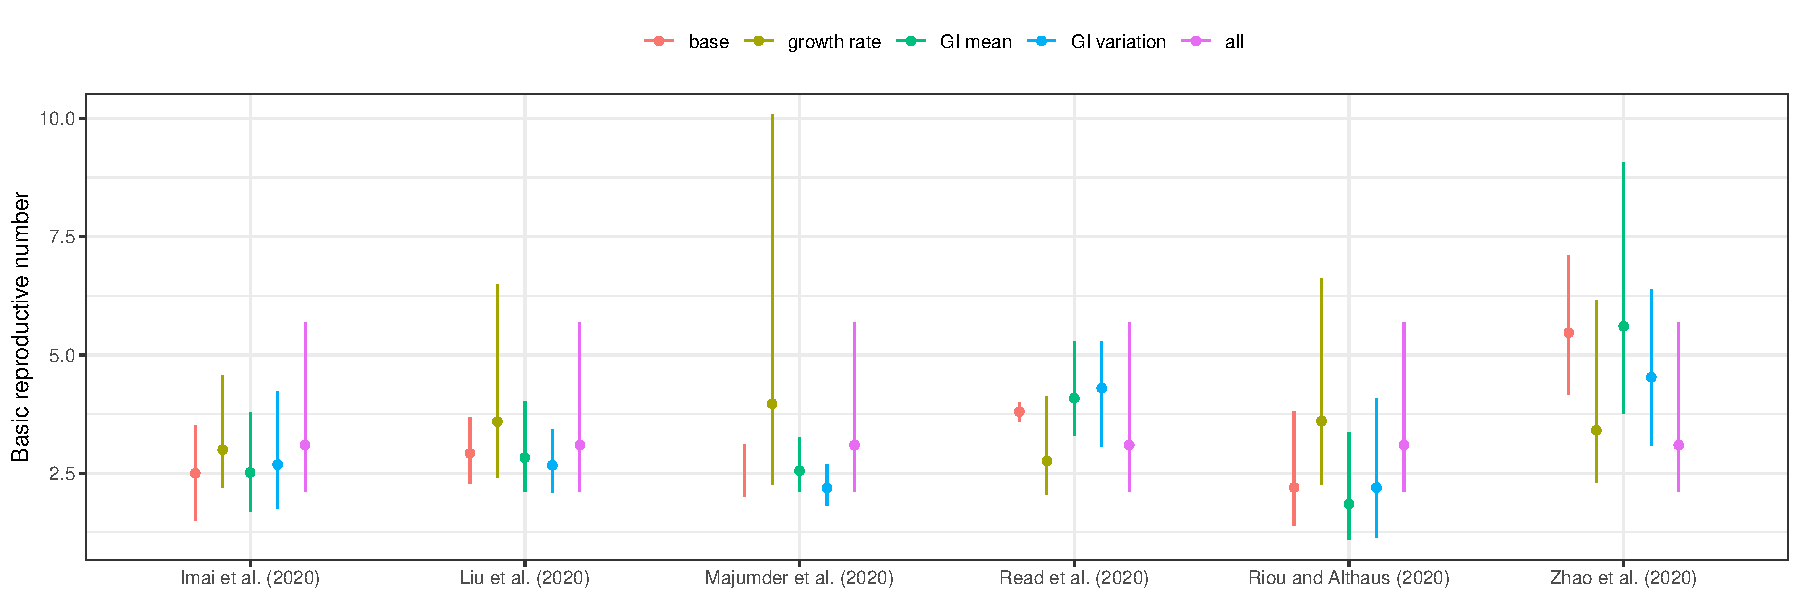
\includegraphics[width=\textwidth]{compare_R0.pdf}
\caption{
\textbf{Sensitivity of the reported \Ro estimates with respect to our pooled estimates of the underlying parameters.}
We replace the reported parameter values (growth rate $r$, GI mean $\bar G$, and GI variation $\kappa$) with our corresponding pooled estimates ($\mu_r$, $\mu_G$, and $\mu_\kappa$) one at a time and recalculate \Ro (\textbf{growth rate}, \textbf{GI mean}, and \textbf{GI variation}).
The pooled estimate of \Ro is calculated from the joint posterior distribution of $\mu_r$, $\mu_G$, and $\mu_\kappa$ (\textbf{all});
this corresponds to replacing all reported parameter values with our pooled estimates, which gives identical results across all studies.
Horizontal dashed lines represent the 95\% confidence intervals of our pooled estimate of \Ro.
The reported \Ro estimates (\textbf{base}) have been adjusted to show the approximate 95\% confidence interval using the probability distributions that we defined if they had relied on different measures for parameter uncertainties.
}
\label{fig:R0}
\end{figure}

Finally, we incorporate all uncertainties by using posterior samples for $\mu_r$, $\mu_G$, and $\mu_\kappa$ to recalculate \Ro and compare it with the reported \Ro estimates.
Our estimated \Ro from the pooled distribution has a median of 3.1 (95\% CI: 2.1--5.7).
While the point estimate of \Ro is similar to other reported values from this date range, the confidence intervals are wider than those of other studies.
This result does not imply that assumptions based on the pooled estimate are too weak;
we believe that this confidence interval more accurately reflects the level of uncertainties present in the information that was available when these models were fitted.
Our median estimate averages over the various studies, and therefore particular studies have higher or lower median estimates.
Here, our focus is on certainty, not on the reason for these discrepancies.
%% JD: WE should add a citation to the model-ensemble literature and say we don't explore but there's some reason to think that the pooled version might be relatively good.

\section{Discussion}

Estimating the basic reproductive number \Ro is crucial for predicting the course of an outbreak and planning intervention strategies.
Here, we used a simple framework \citep{park2019practical} to compare estimates of \Ro for the novel coronavirus outbreak.
Our results demonstrate the importance of accounting for uncertainties associated with the underlying generation-interval distributions, including with the amount of dispersion in the generation intervals:
although our pooled estimates are relatively insensitive to the estimated uncertainty, our analysis of individual studies shows that assuming too narrow a generation-interval distribution can make the estimate of \Ro too sensitive to the estimates of the exponential growth rate $r$.

In this study, we focused on propagating errors arising from implicit or explicit estimates of growth rate and generation intervals. Other key issues underlying early estimates of \Ro\ include statistical independence and types of noise. 

Of the six studies that we reviewed, two of them directly fit their models to cumulative number of confirmed cases.
This approach can be appealing because of its simplicity and apparent robustness, but fitting a model to cumulative incidence instead of raw incidence can both bias parameters and give overly narrow confidence intervals, if the result non-independent error structures are not taken into account \citep{ma2014estimating, king2015avoidable}.
Naive fits to cumulative incidence data should be avoided.

There are many real-world sources of noise in real-world incidence data, including both dynamical, or ``process'', noise (randomness that directly or indirectly affects disease transmission); and observation noise (randomness underlying how many of the true cases are reported).  
Disease modelers face the choice of incorporating one or both of these in their data-fitting and modeling steps. 
This is not always a serious problem, particularly if the goal is inferring parameters rather than directly making forecasts (e.g., \citep{ma2014estimating}).
Modelers should be aware of the possibility that ignoring one kind of error can give overly narrow confidence intervals (e.g., \citep{king2015avoidable}).

Here, we focused on the estimates of \Ro that were published within a very short frame of time (January 24th--26th).
Although our analysis only reflects a snapshot of a fast-moving epidemic, our lessons will hold: confidence intervals must combine different sources of uncertainty. 
In fact, as epidemics progress and more data becomes available, it is likely that inferences about exponential growth rate will become more precise; thus the risk of over-confidence when uncertainty about the generation-interval distribution is neglected will become greater.

We strongly emphasize the value of attention to accurate characterization of the transmission chains via contact tracing and better statistical framework for inferring generation-interval distributions from such data \citep{britton2019estimation}.
A combined effort between public-health workers and modelers in this direction will be crucial for predicting the course of an epidemic and controlling it.
We also emphasize the value of transparency from modelers.
Model estimates during an outbreak, even in pre-prints, should include code links and complete explanations.
Ideally, the code should not rely on closed-source programs.

We have provided a basis for evaluating and comparing exponential-growth based estimates of \Ro\ in terms of three simple components: the exponential growth rate, mean generation interval, and generation interval dispersion. We are hopeful that this will provide a guide to understanding and reconciling different estimates early in an epidemic.

\section{Methods}

\subsection{Gamma approximation framework for linking $r$ and $\mathcal R_0$}

Early in an outbreak, \Ro is difficult to estimate directly;
instead, \Ro is often inferred from the exponential growth rate $r$, which can be estimated reliably from incidence data \citep{mills2004transmissibility, nishiura2009transmission, ma2014estimating}.
Given an estimate of the exponential growth rate $r$ and an \emph{intrinsic} generation-interval distribution $g(\tau)$ \citep{champredon2015intrinsic}, the basic reproductive
number can be estimated via the Euler-Lotka equation \citep{wallinga2007generation}:
\begin{linenomath*}
\begin{equation}
1/\mathcal R_0 = \int \exp(-r\tau) g(\tau) d\tau.
\label{eq:euler}
\end{equation}
\end{linenomath*}
In other words, estimates of \Ro must
depend on the assumptions about the
exponential growth rate $r$ and the shape of the generation-interval distribution $g(\tau)$.

Here, we use the gamma approximation framework \citep{mcbryde2009early, nishiura2009transmission, roberts2011early, park2019practical} to (1) characterize the amount of uncertainty present in the exponential growth rates and the shape of the generation-interval distribution and (2) assess the degree to which these uncertainties affect the estimate of \Ro.
Assuming that generation intervals follow a gamma distribution
with the mean $\bar G$ and the squared coefficient of variation (CV$^2$) $\kappa$, 
we have
\begin{linenomath*}
\begin{equation}
\mathcal R_0 = \left(1 + \kappa r \bar{G}\right)^{1/\kappa}.
\label{eq:gamma}
\end{equation}
\end{linenomath*}
This equation demonstrates that a generation-interval distribution
that has a larger mean (higher $\bar{G}$) or is less variable (lower $\kappa$)
will give a higher estimate of \Ro for the same value of $r$.

\subsection{Description of the studies}

We reviewed 6 modeling studies of the novel coronavirus outbreak that were published online between January 24th, 2020 and January 26th, 2020 (Table 1).
Five studies \citep{liuncov, majumderncov, readncov, riouncov, zhaoncov} were uploaded to preprint servers (bioRxiv, medRxiv, and SSRN), and one report was posted on the website of Imperial College London \citep{imaincov}.
There is a wide variation in their statistical methods and the amount of data they used to infer \Ro.
\cite{imaincov} and \cite{riouncov} simulated branching process models and compared the predicted number of cases from their models with the estimated number of total cases by January 18th.
\cite{readncov} fitted a deterministic, metapopulation Susceptible-Exposed-Infected-Recovered (SEIR) model to incidence data between January 1st and January 21st from major cities in China and other countries.
\cite{zhaoncov} and \cite{liuncov} fitted exponential growth models to incidence data up to January 22nd and January 23rd, respectively, and inferred \Ro\ via the Euler-Lotka equation (\eref{euler}).
\cite{majumderncov} fitted the Incidence Decay and Exponential Adjustment (IDEA) model \citep{fisman2013idea} to incidence data up to January 26th, which is equivalent to fitting an exponential growth model and assuming a fixed generation-interval distribution.

\subsection{Statistical framework}

For each study, we construct a family of parameter sets by drawing 100,000 random samples from the probability distributions (Table 2) that represent the estimates of \Ro and the assumed values of $\bar G$ and $\kappa$ and calculating the exponential growth rate $r$ via the inverse of \eref{gamma}:
\begin{linenomath*}
\begin{equation}
r_i = \frac{{\mathcal R_{0i}}^{\kappa_i} - 1}{\kappa_i \bar{G}_i}.
\end{equation}
\end{linenomath*}
This allows us to approximate the probability distributions of the estimated exponential growth rates by each study;
uncertainties in the probability distributions that we calculate for the estimated exponential growth rates will reflect the methods and assumptions that the studies rely on.

We construct pooled estimates for each parameter ($r$, $\bar G$, and $\kappa$) using a Bayesian multilevel modeling approach, which assumes that the parameters across different studies come from the same gamma distribution:
\begin{linenomath*}
\begin{equation}
\begin{aligned}
r_i &\sim \gammdist(\mathrm{mean}=\mu_r, \mathrm{shape}=\alpha_r),\\
\bar{G}_i &\sim \gammdist(\mathrm{mean}=\mu_G, \mathrm{shape}=\alpha_G),\\
\kappa_i &\sim \gammdist(\mathrm{mean}=\mu_\kappa, \mathrm{shape}=\alpha_\kappa).\\
\end{aligned}
\end{equation}
\end{linenomath*}
We account for uncertainties associated with $r_i$, $\bar G_i$ and $\kappa_i$ (and their correlations), by drawing a random set from the family of parameter sets for each study at each Metropolis-Hastings step;
this approach is analogous to Bayesian methods for analyzing phylogenetic data, which often rely on drawing random samples of phylogenetic trees from a discrete set to account for phylogenetic uncertainty \citep{pagel2004bayesian,bedford2014integrating}.
Since the gamma distribution does not allow zeros, we use $\kappa =0.02$ instead for Study 6.

Weakly informative priors are assumed on the hyperparameters:
\begin{linenomath*}
\begin{equation}
\begin{aligned}
\mu_r &\sim \gammdist(\mathrm{mean}=1\,\mathrm{week}^{-1},\,\mathrm{shape}=0.1)\\
\mu_G &\sim \gammdist(\mathrm{mean}=1\,\mathrm{week},\,\mathrm{shape}=0.1)\\
\mu_\kappa &\sim \gammdist(\mathrm{mean}=0.5,\,\mathrm{shape}=0.1)\\
(\alpha_r, \alpha_G, \alpha_\kappa) &\sim \gammdist(\mathrm{mean}=1,\,\mathrm{shape}=0.1).
\end{aligned}
\end{equation}
\end{linenomath*}
We run 4 parallel Markov Chain Monte Carlo (MCMC) chains that consist of 200,000 burnin steps and 200,000 sampling steps.
Posterior samples are thinned every 400 steps.
Convergence is assessed by ensuring that the Gelman-Rubin statistic is below 1.01 for all hyperparameters \citep{gelman1992inference}.
95\% confidence intervals are calculated by taking 2.5\% and 97.5\% quantiles from the posterior distribution.
\texttt{R} code is available in GitHub (https://github.com/parksw3/nCoV\_framework).

\section*{Acknowledgements}

We thank Ben Bolker for providing useful comments on the manuscript.

\pagebreak

\bibliography{wuhan}

\end{document}
